\chapter{Implementation}

\section{Building a Basic Game Environment}

My first task was to build a basic game environment within Godot that could then be built further upon.
This consists of:
\begin{itemize}
    \item \textbf{Player Character}: I implemented a character with basic movement controls including running left/right, jumping, and falling with appropriate physics, using Godot's built in 2D physics system.
    \item \textbf{Camera}: The game's camera is a Camera2D node that remains static providing a view of the whole map.
    \item \textbf{Tile Based Map}: I created a tilemap system using Godot's TileMapLayer node, allowing me to construct levels from reusable tiles representing walls, floors and ceilings.
    \item \textbf{Kill Plane}: At the bottom of the map, there is a player collidable box that will reset their position if it is touched. This ensures that the player cannot fall out of the map endlessly.
    \item \textbf{Finish Line and Timer}: Each map contains a finish line tile. As soon as the player is instantiated, their timer starts and will stop once they touch the finish line.
\end{itemize}

\begin{figure}[H]
    \centering
    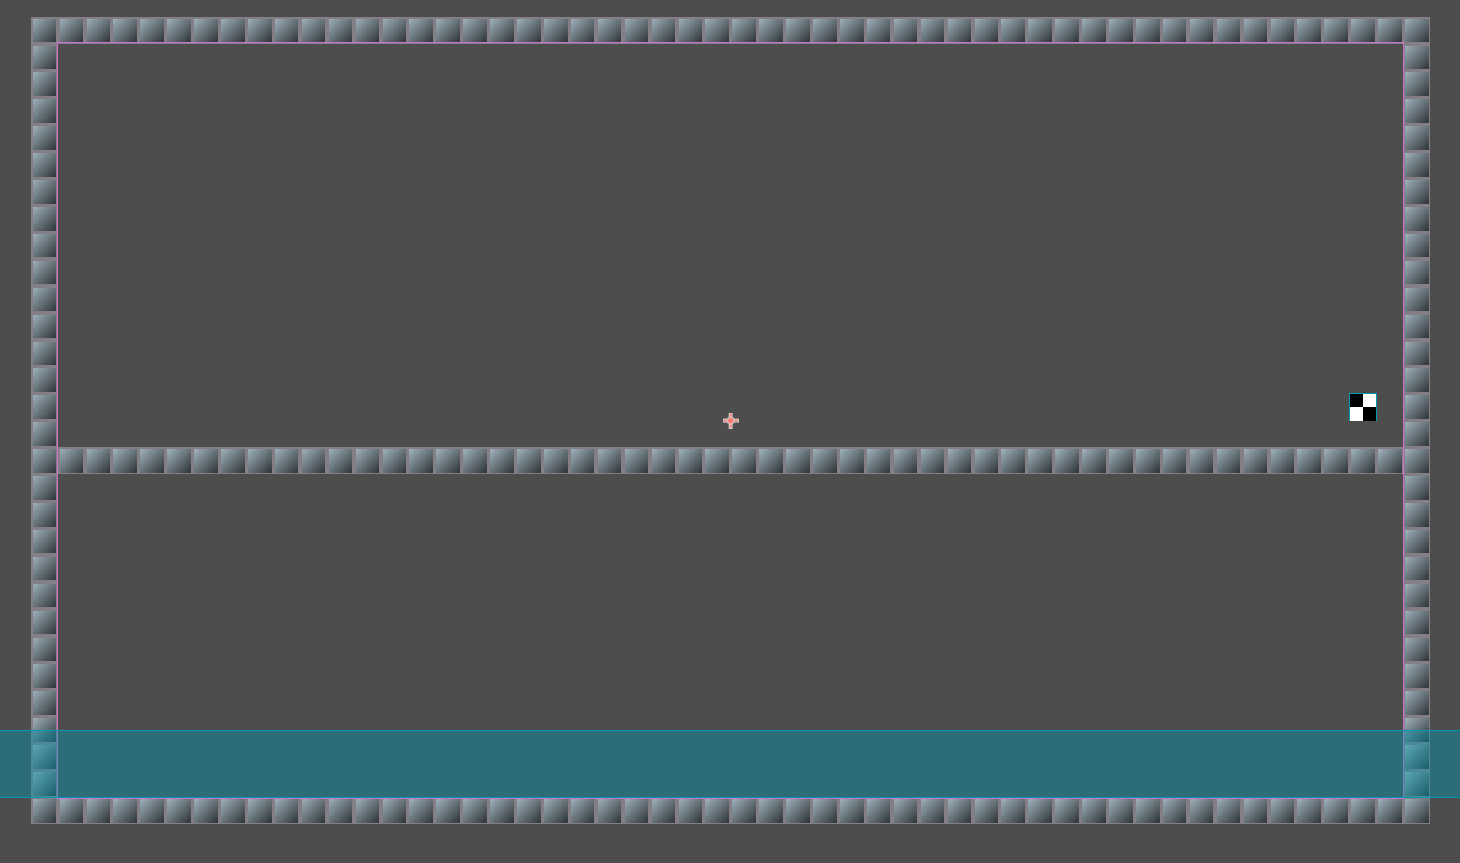
\includegraphics[width=0.8\textwidth]{figures/godot_environment_basic}
    \caption{Basic Godot game environment}
    \label{fig:godot_environment_basic}
\end{figure}

Godot's node based architecture allowed me to neatly lay these all out.

\begin{figure}[H]
    \centering
    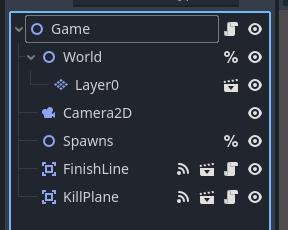
\includegraphics[width=0.8\textwidth]{figures/godot_nodes_basic.png}
    \caption{Environment's node hierarchy}
    \label{fig:godot_nodes_basic}
\end{figure}

Building upon this foundational environment, I implemented a separate AI Player node to serve as the agent controlled by the reinforcement learning model. 
This AI Player functions as a physics-affected body with identical physical properties to the player character, ensuring that both human and AI participants operate under the same environmental constraints. 
The key distinction is that while the human player responds to keyboard or controller inputs, the AI Player receives its movement commands exclusively from the reinforcement learning model via the network communication system. 
The separate node implementation also facilitates the competitive gameplay structure, allowing the AI to demonstrate a complete run before the human player attempts the same procedurally generated level.
To facilitate the training process, the AI Player keeps track of "stuck time". This is a counter that starts counting up if the AI has not made horizontal progress towards the goal. 
After 2 seconds have elapsed, the AI is reset to it's starting point and a fail is counted. This helps the training process as I would often find that the model would get stuck during the early stages of training.

\subsection{Procedural Map Generation}

To evaluate the agent's adaptability across diverse environments, I implemented a procedural map generation system that could create varied challenge scenarios. This system produces three distinct map types:

\begin{itemize}
    \item \textbf{Pillars}: Generates vertical obstacles of variable height and width between the player starting position and the goal. This design tests the agent's ability to navigate vertical challenges through precise jumping.
    \item \textbf{Snake}: Creates a randomised horizontal tunnel pathway that winds between the starting position and the goal. This configuration evaluates the agent's capacity to follow constrained paths.
    \item \textbf{Platforms}: Places discontinuous platforms at randomised heights across the map. This challenging layout requires the agent to make calculated jumps between platforms while avoiding fatal falls through the gaps.
\end{itemize}

The procedural generation system ensures that each training episode presents the agent with a unique layout while maintaining consistent difficulty parameters. 
This approach prevents the model from simply memorising specific map solutions and instead encourages the development of generalised navigation strategies.
The map type can be selected by the user from the main menu with a drop down selector box.

\begin{figure}[H]
    \centering
    \begin{minipage}{0.32\textwidth}
        \centering
        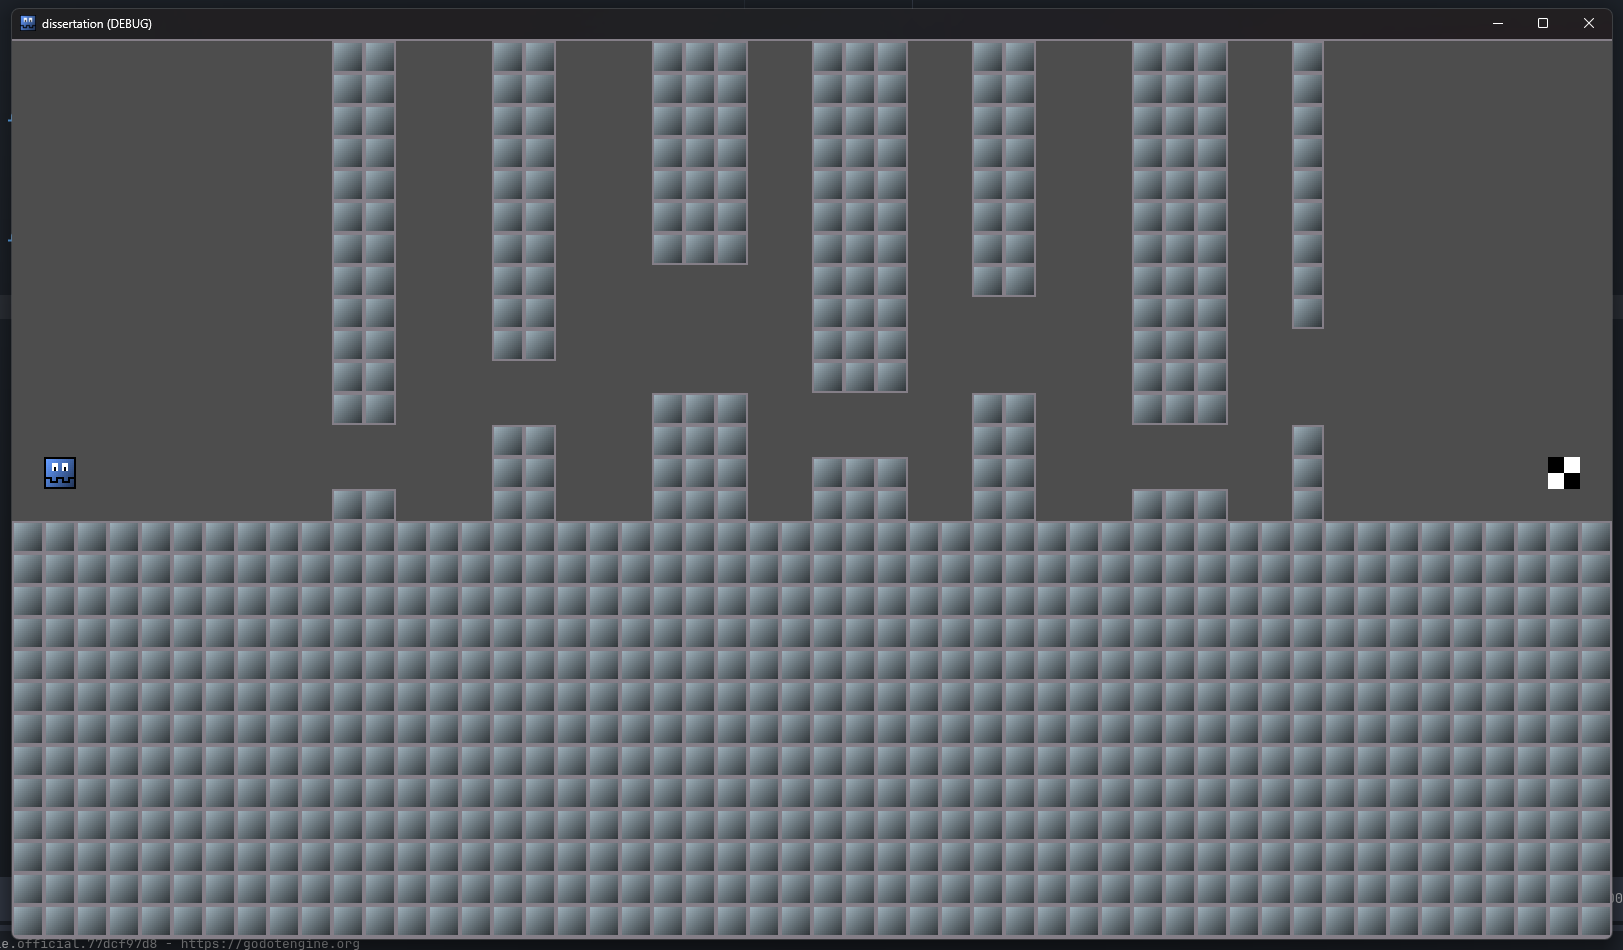
\includegraphics[width=\linewidth]{figures/pillars}
        \caption{Pillars}
        \label{fig:pillars}
    \end{minipage}
    \hfill
    \begin{minipage}{0.32\textwidth}
        \centering
        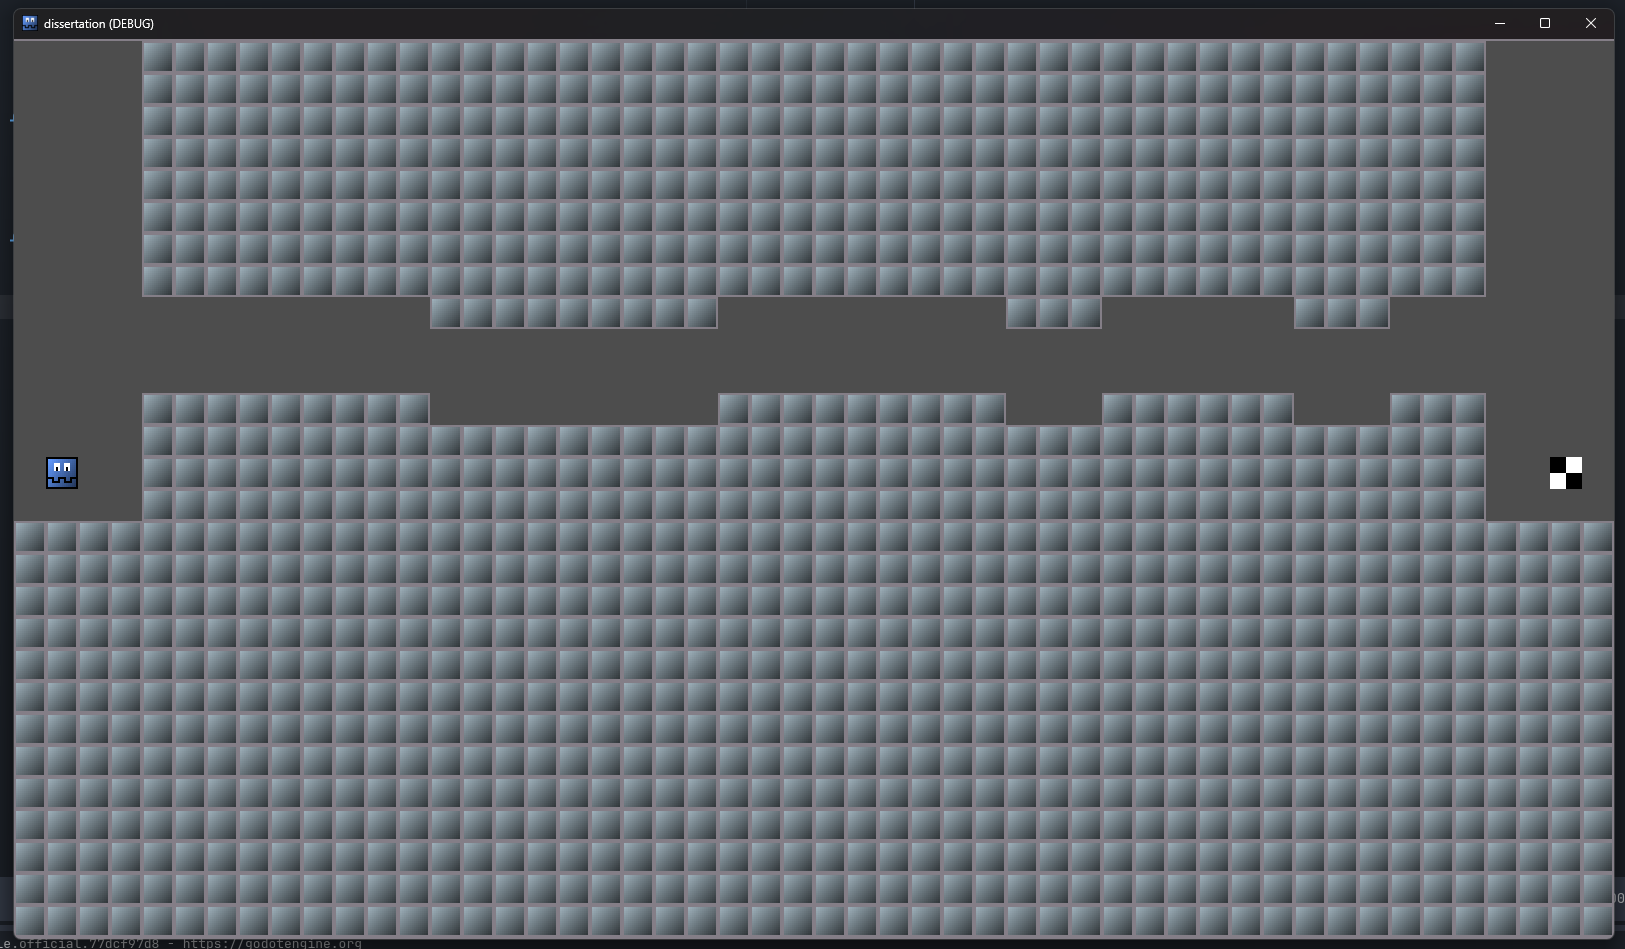
\includegraphics[width=\linewidth]{figures/snake}
        \caption{Snake}
        \label{fig:snake}
    \end{minipage}
    \hfill
    \begin{minipage}{0.32\textwidth}
        \centering
        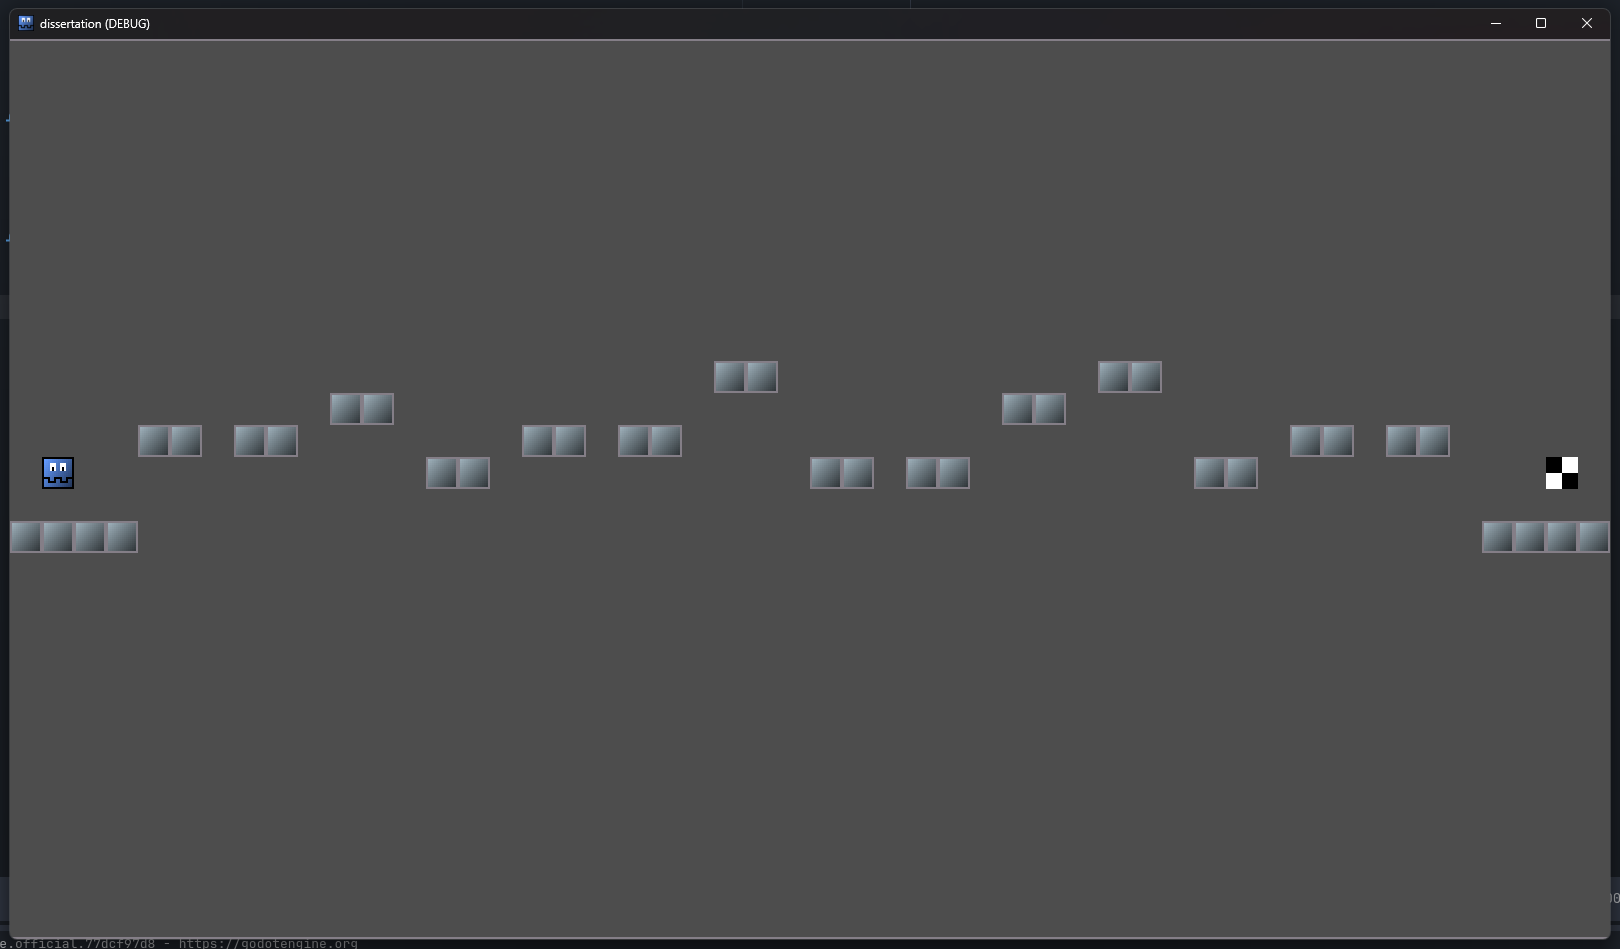
\includegraphics[width=\linewidth]{figures/platforms}
        \caption{Platforms}
        \label{fig:platforms}
    \end{minipage}
    \caption{Procedurally generated map types}
    \label{fig:map_types}
\end{figure}

\section{Debug Information}

To facilitate the development process, I implemented comprehensive debug information within the game environment. 
This included a visual representation of the agent's current observation state, allowing direct inspection of what the model "sees" from the 7×7 grid centered on its position. 
Distance metrics were also continuously displayed, showing the agent's proximity to the goal and enabling real-time evaluation of progress. 
Additional timing metrics were incorporated to track performance data relevant to the agent's decision-making processes. 
These debugging tools proved invaluable during development, providing immediate visual feedback on the observation system's functionality and the agent's environmental perception.
These features can be toggled via a switch on the main menu.

\begin{figure}[H]
    \centering
    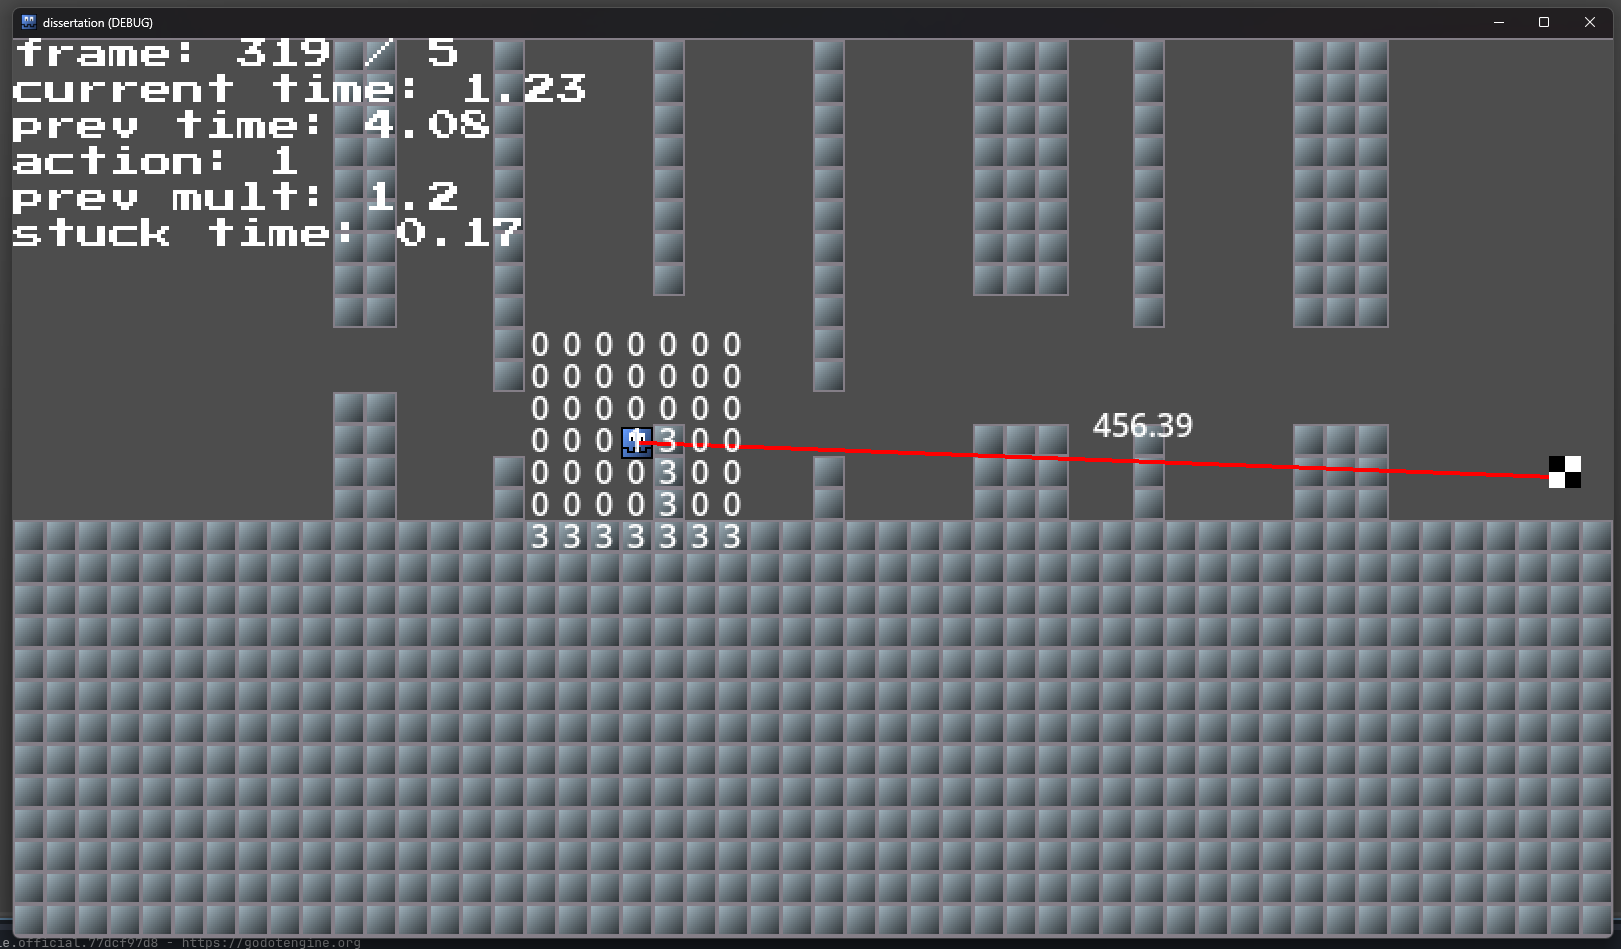
\includegraphics[width=0.8\textwidth]{figures/debug_info}
    \caption{Game running with debug information turned on}
    \label{fig:debug_info}
\end{figure}

\section{State Observation System}

For the reinforcement learning agent to make informed decisions, it needs to perceive its environment effectively. 
This required designing an observation system attached to the AI Player that captures relevant environmental information while maintaining computational efficiency.

\subsection{Observation Scope and Representation}

While capturing the entire environment state would provide the agent with complete information, such an approach proved prohibitively expensive from a computational perspective. A full environment representation would
significantly increase the input dimensionality of the neural network, require substantially more training time to converge, demand greater memory resources during both training and inference, and scale poorly with larger environment sizes. 
These computational constraints led me to pursue a more efficient observation approach that would balance environmental awareness with practical implementation considerations.

After experimentation with various observation window sizes, I determined that a 7×7 grid centered on the player offered an optimal balance between environmental awareness and computational efficiency. 
This window size provides sufficient context about nearby obstacles, pathways, and goals while keeping the state representation compact and manageable. 
The constrained field of view also encourages the agent to develop more generalizable navigation strategies rather than memorising specific map layouts, potentially improving transfer learning capabilities across different environments.
The agent perceives a 7×7 grid centered on its position, providing sufficient contextual awareness of the immediate surroundings.

This observation window uses a simple numerical encoding scheme:
\begin{itemize}
    \item \textbf{0}: Empty space / traversable areas 
    \item \textbf{1}: Player character (Always at the centre of the grid)
    \item \textbf{2}: Finish line
    \item \textbf{3}: Walls / non-traversable terrain
\end{itemize}

\begin{figure}[H]
    \centering
    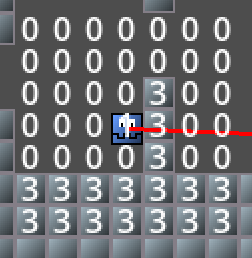
\includegraphics[width=0.8\textwidth]{figures/observation_window}
    \caption{Visualisation of the observation window}
    \label{fig:observation_window}
\end{figure}

\subsection{Implementation Mechanics}

The observation mechanism operates on each frame update, scanning the surrounding tiles relative to the agent's position. 
For each coordinate within the 7×7 grid, the system queries the tilemap to determine the tile type at that location. 
This information is then encoded according to the numerical scheme and assembled into an array.
This process is run twice, once for the initial observation, and again for the second observation used alongside the reward.

This representation offers several advantages:
\begin{itemize}
    \item \textbf{Translation invariance}: The agent learns based on relative positions rather than absolute map coordinates
    \item \textbf{Computational efficiency}: The fixed-size input simplifies network architecture and reduces processing requirements
    \item \textbf{Informational clarity}: The categorical encoding provides clear distinctions between critical environmental features
\end{itemize}

Once constructed, this state representation is transmitted to the reinforcement learning model, which uses it as input for determining the next optimal action. 

\section{Determining reward}
Designing an effective reward function was critical for the reinforcement learning agent's success. After extensive experimentation, I implemented a straightforward distance-based reward mechanism that provides immediate feedback after each action:

\begin{itemize}
    \item \textbf{+1 reward} when the agent moves closer to the finish line
    \item \textbf{-1 penalty} when the agent moves further from the finish line
    \item \textbf{+1.2/0.8 additional reward} upon reaching the goal. The higher reward is granted when the agent reaches the goal faster than the previous attempt, and vice versa.
\end{itemize}

This reward function is run once each frame, alongside the second observation, after the model has made an action.

This simple approach encourages the agent to make continuous progress toward the objective while maintaining computational efficiency. 
The reward function balances immediate guidance with the freedom to discover optimal paths independently.
During development, I explored several alternative reward structures, including proportional multipliers (×1.2/×0.8) and larger magnitude rewards (+600 for goal completion, -300 for falling). 
However, these higher values led to training instability, causing the model to struggle with convergence. The proportional multipliers proved beneficial and were retained, while the reward magnitudes were scaled back to ±1 to ensure stable learning.
I also experimented with line-of-sight rewards using raycasting techniques, where the agent would receive additional rewards when establishing visual contact with the goal. 
After testing, this approach was ultimately not incorporated into the final implementation as it did not significantly improve performance while adding computational overhead.

A significant limitation of this reward structure is that it discourages exploratory backtracking, effectively requiring level designs to maintain a linear progression toward the goal. 
This constraint arises because the agent receives consistent penalties when moving away from the finish line, even when such movements might be strategically necessary to navigate complex environmental features. 
While this simplifies the learning process for straightforward courses, it potentially limits the agent's ability to discover optimal solutions in more complex, non-linear environments where temporary retreat may be advantageous.

\section{Implementing Networking}

To facilitate communication between the Godot game environment and the Python-based reinforcement learning model, I developed a robust networking system using TCP sockets and JSON encoding. 
This approach allows the game state to be effectively transmitted to the model for processing, and action decisions to be received back for execution within the game environment.

\subsection{Communication Protocol Design}

After evaluating several options for inter-process communication, I selected a TCP socket-based approach with JSON encoding for several key reasons:

\begin{itemize}
    \item \textbf{Reliability}: TCP's connection-oriented nature ensures that no state observations or action commands are lost during transmission
    \item \textbf{Cross-platform compatibility}: The socket-based approach works seamlessly across different operating systems. The JSON encoding also ensures that the state and reward data is encoded and decoded the same on both the Godot side and the Python side.
    \item \textbf{Low implementation overhead}: Both Godot and Python offer built-in libraries for TCP communication without requiring additional dependencies
\end{itemize}

To implement this, I used the \textit{socket} library on the python side, and a \textit{StreamPeerTCP} node on the Godot side.

\subsection{Operational Modes}

The Python component of the system was designed with two distinct operational modes:

\begin{itemize}
    \item \textbf{Training Mode}: Incorporates epsilon-greedy exploration strategies and periodically saves model checkpoints to preserve training progress. This mode focuses on model improvement through experience gathering and optimisation.
    \item \textbf{Play Mode}: Loads the latest saved checkpoint and plays deterministically with epsilon set to zero, demonstrating the current capabilities of the trained model without further exploration.
\end{itemize}

\subsection{Communication Cycle Implementation}

As we are working within a game context, to get the state and reward from any given action, we must wait until the next frame of the game for the result of the action to be processed. 

The core networking loop on the Godot side follows a structured pattern of state transmission and action reception:

\begin{enumerate}
    \item First, the game engine calculates and sends the reward from the previous action along with the current state observation
    \item It then awaits confirmation that the Python script is ready for the next cycle
    \item Upon confirmation, the game sends a fresh observation of the current environment state
    \item Finally, it receives the model's selected action (encoded as an integer: 0 for left movement, 1 for right movement, 2 for jump) and executes this action within the game environment
\end{enumerate}

This communication cycle repeats once each frame during gameplay, maintaining a consistent feedback loop between the game environment and the learning model. 
The implementation ensures that state observations, rewards, and actions are synchronised properly, preventing timing issues that could otherwise lead to misaligned learning experiences.

The code excerpt below illustrates the essential communication pattern written in GDScript:

\singlespaced
\begin{verbatim}
    # Transmit previous reward and current state
    var model_reward : float = reward()
    peer.put_float(model_reward)
    peer.poll()
    var next_state : Dictionary = observe()
    var next_state_encoded : PackedByteArray = 
        JSON.stringify(next_state).to_utf8_buffer()
    peer.put_data(next_state_encoded)
    peer.poll()

    # Await ready signal from Python
    peer.poll()
    var _isready : String = peer.get_string(5)

    # Send observation for decision making
    var visibleTiles : Dictionary = observe()
    var visibleTilesEncoded : PackedByteArray = 
        JSON.stringify(visibleTiles).to_utf8_buffer()
    peer.put_data(visibleTilesEncoded)
    peer.poll()

    # Receive and execute model's action decision
    peer.poll()
    var model_action : int = peer.get_u8()
    action(delta, model_action)
\end{verbatim}
\doublespaced

This networking implementation provides the critical infrastructure that allows the reinforcement learning agent to interact with the game environment, facilitating the entire learning process.

\section{Implementing the Model}

For the reinforcement learning component, I implemented a Deep Q-Network (DQN) architecture with convolutional layers to process the spatial information from the game environment.

\subsection{Model Architecture}

After considering various neural network architectures, I selected a convolutional DQN model that could efficiently process the 2D grid observation data from the game environment:

\begin{itemize}
    \item \textbf{Input Layer}: Accepts the 7×7 grid observation (49 values) reshaped into a 2D format.
    \item \textbf{Convolutional Layer}: A 2D convolutional layer with 16 filters, kernel size of 3×3, stride of 1, and padding of 1, enabling the network to detect spatial patterns in the environment.
    \item \textbf{Hidden Layers}: Two fully-connected layers with 128 neurons each and ReLU activation functions.
    \item \textbf{Output Layer}: A fully-connected layer with 4 outputs corresponding to the possible actions (move left, move right, jump, do nothing).
\end{itemize}

The convolutional layer was particularly important for this implementation as it allows the model to recognise patterns in the spatial arrangement of walls, empty spaces, and the goal within the observation window. 
This spatial awareness is critical for navigating the platformer environment effectively. Below is a code listing of the Pytorch model definition.
\singlespaced
\begin{verbatim}
    class DQN(nn.Module):
    def __init__(self, n_observations, n_actions):
        super(DQN, self).__init__()
        # Reshape the input for Conv2D
        self.input_dim = int(np.sqrt(n_observations))
        
        # Convolutional layer
        self.conv1 = nn.Conv2d(1, 16, kernel_size=3, stride=1, padding=1)
        
        # Calculate the size after convolution for the fully connected layer
        conv_output_size = 16 * self.input_dim * self.input_dim
        
        self.fc1 = nn.Linear(conv_output_size, 128)
        self.fc2 = nn.Linear(128, 128)
        self.fc3 = nn.Linear(128, n_actions)
        
    def forward(self, x):
        # Reshape input to [batch_size, channels, height, width]
        batch_size = x.size(0)
        x = x.view(batch_size, 1, self.input_dim, self.input_dim)
        
        # Apply convolution and activation
        x = F.relu(self.conv1(x))
        
        # Flatten for fully connected layers
        x = x.view(batch_size, -1)
        
        x = F.relu(self.fc1(x))
        x = F.relu(self.fc2(x))
        x = self.fc3(x)
        return x
\end{verbatim}
\doublespaced

\subsection{Training Algorithm}

I implemented a standard Q-learning algorithm with a target network for stable training. 
The training strategy incorporated several key techniques to enhance learning and stability. 
Epsilon-greedy exploration was implemented, beginning with a high exploration rate that gradually decreased over time, creating an effective balance between exploring new strategies and exploiting learned knowledge. 
This approach allowed the agent to discover potentially valuable actions early in training while increasingly focusing on optimal strategies as training progressed. 
A target network was employed as a separate network with parameters periodically updated from the main network, providing stable Q-value targets during training and mitigating the risk of divergence that can occur in Q-learning when the same values are both predicted and used as training targets.
The Adam optimiser was selected with a learning rate of 0.001 for its adaptive learning rate capabilities, allowing for efficient parameter updates that dynamically adjusted based on gradient history. 
This optimiser helped navigate the complex loss landscape more effectively than traditional stochastic gradient descent. 
Finally, Mean Squared Error was used as the loss function between predicted Q-values and target Q-values, providing a differentiable metric that penalised large prediction errors more heavily, guiding the network toward more accurate action-value estimations and ultimately more optimal decision-making policies.

\subsubsection{Replay Buffer}

I implemented an experience replay buffer to enhance training stability and efficiency. 
This buffer stores transitions (state, action, reward, next\_state) as the agent interacts with the environment:

\singlespaced
\begin{verbatim}
class ReplayMemory(object):
    def __init__(self, capacity):
        self.memory = deque([], maxlen=capacity)
    
    def push(self, state, action, next_state, reward):
        self.memory.append((state, action, next_state, reward))
    
    def sample(self, batch_size):
        return random.sample(self.memory, batch_size)
    
    def __len__(self):
        return len(self.memory)
\end{verbatim}
\doublespaced

However, after extensive testing, I found that in this specific implementation, the replay buffer provided minimal benefits. 
The relative simplicity of the environment and model architecture meant that the agent achieved sufficient performance through direct online updates. 
Furthermore, with the limited training duration in the experimental setting, the buffer rarely reached capacity before training concluded. 
This observation aligns with research suggesting that for simpler environments with limited state spaces, the overhead of experience replay may not always justify its benefits.

\subsection{Training Process}

The training process operated on a cycle-by-cycle basis with the game environment:

\begin{enumerate}
    \item Receive the current state observation from the Godot environment
    \item Select an action using the epsilon-greedy policy
    \item Send the selected action to the game environment for execution
    \item Receive the reward and next state observation
    \item Update the Q-network.
    \item Periodically update the target network parameters
\end{enumerate}

During training, the epsilon value (controlling exploration vs. exploitation) decayed from an initial value of 0.9 to a minimum of 0.1, 
allowing the agent to gradually transition from predominantly random exploration to informed decision-making based on learned values.

\subsection{Model Checkpointing}

To ensure training progress was preserved across sessions and allow for model evaluation at different training stages, I implemented a model checkpointing system. 
At regular intervals during training (every 1000 iterations), the system automatically creates a checkpoint file containing the complete model state. 
These checkpoint files store the current iteration count to preserve the exact position in the training sequence, the model state dictionary containing the complete set of weights and biases for the neural network, the states from the optimiser, the most recent loss value for performance evaluation, and the current epsilon value which maintains the proper exploration/exploitation balance. 
Each checkpoint is saved with a unique filename incorporating the iteration number, creating a traceable history of the model's evolution throughout training. This systematic approach provides several key benefits: it safeguards against potential training interruptions, enables training to resume from intermediate points without starting over, facilitates comparative analysis between different training stages, and supplies ready-to-use models for the play mode implementation.


\section{Integration of AI into Gameplay}

The final integration of the AI component into gameplay implements a straightforward competitive framework. The system follows a simple procedural flow:
The game procedurally generates a new stage layout when a level begins. 
First, the AI agent performs a complete navigation run through this generated environment, establishing a baseline completion time. 
Following the agent's run, the player is then challenged to complete the identical stage, with the AI's performance time presented as the target to beat. 
This implementation creates a direct competitive dynamic between human and artificial intelligence performance. 
While time constraints limited the development of more sophisticated integration features, this approach effectively demonstrates the practical application of the reinforcement learning model within an actual gameplay context.
The competition framework provides an intuitive way for players to benchmark their skills against the trained agent, while also showcasing the agent's capabilities across the procedurally generated environments.
